\section{Portal by example}
\label{sec:language}

\begin{figure}[t!]
\centering
  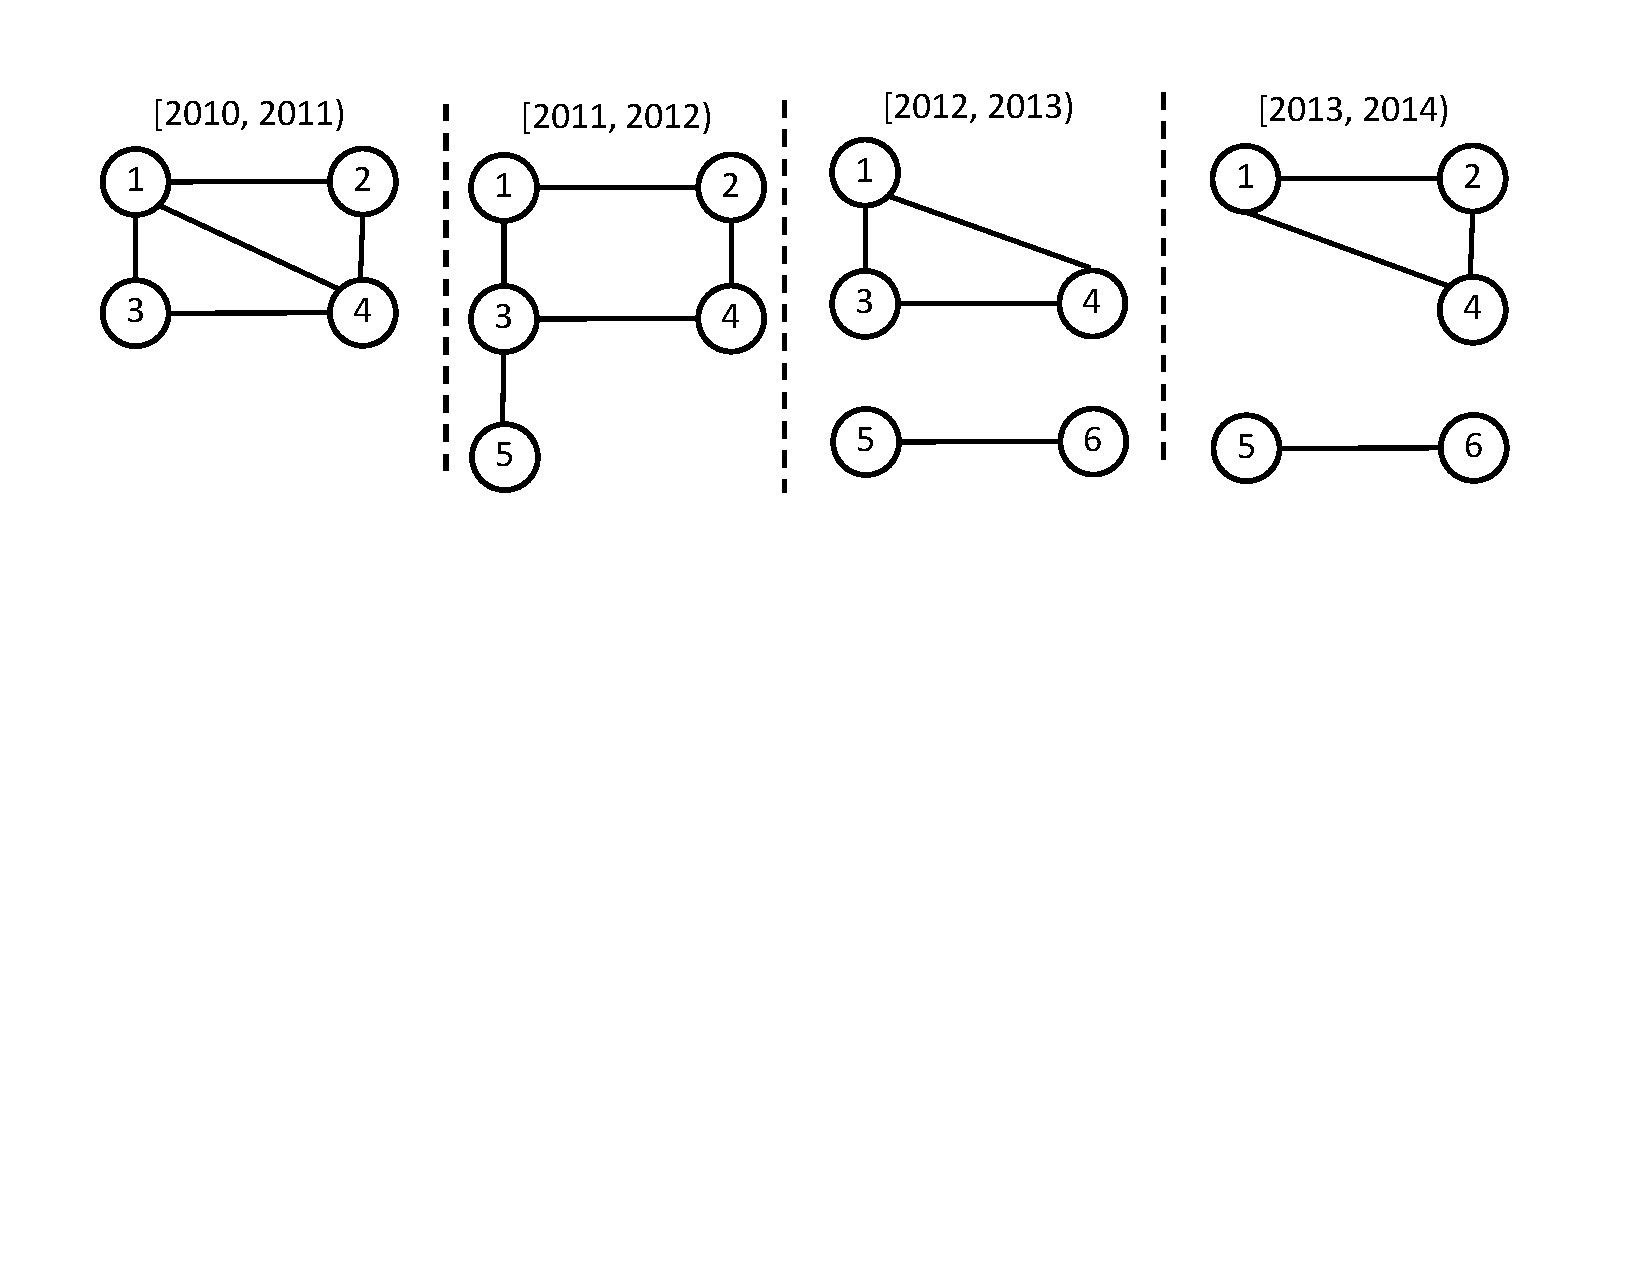
\includegraphics[width=2.9in]{figs/4snaps_T1.pdf}
  \caption{\tg \insql{T1} with 4 snapshots.}
  \vspace{-0.5cm}
  \label{fig:tg_t1}
  \vspace{-0.2cm}
\end{figure}

\eat{
\begin{figure*}[th!]
\centering
\begin{minipage}{3.2in}
 % \centering
  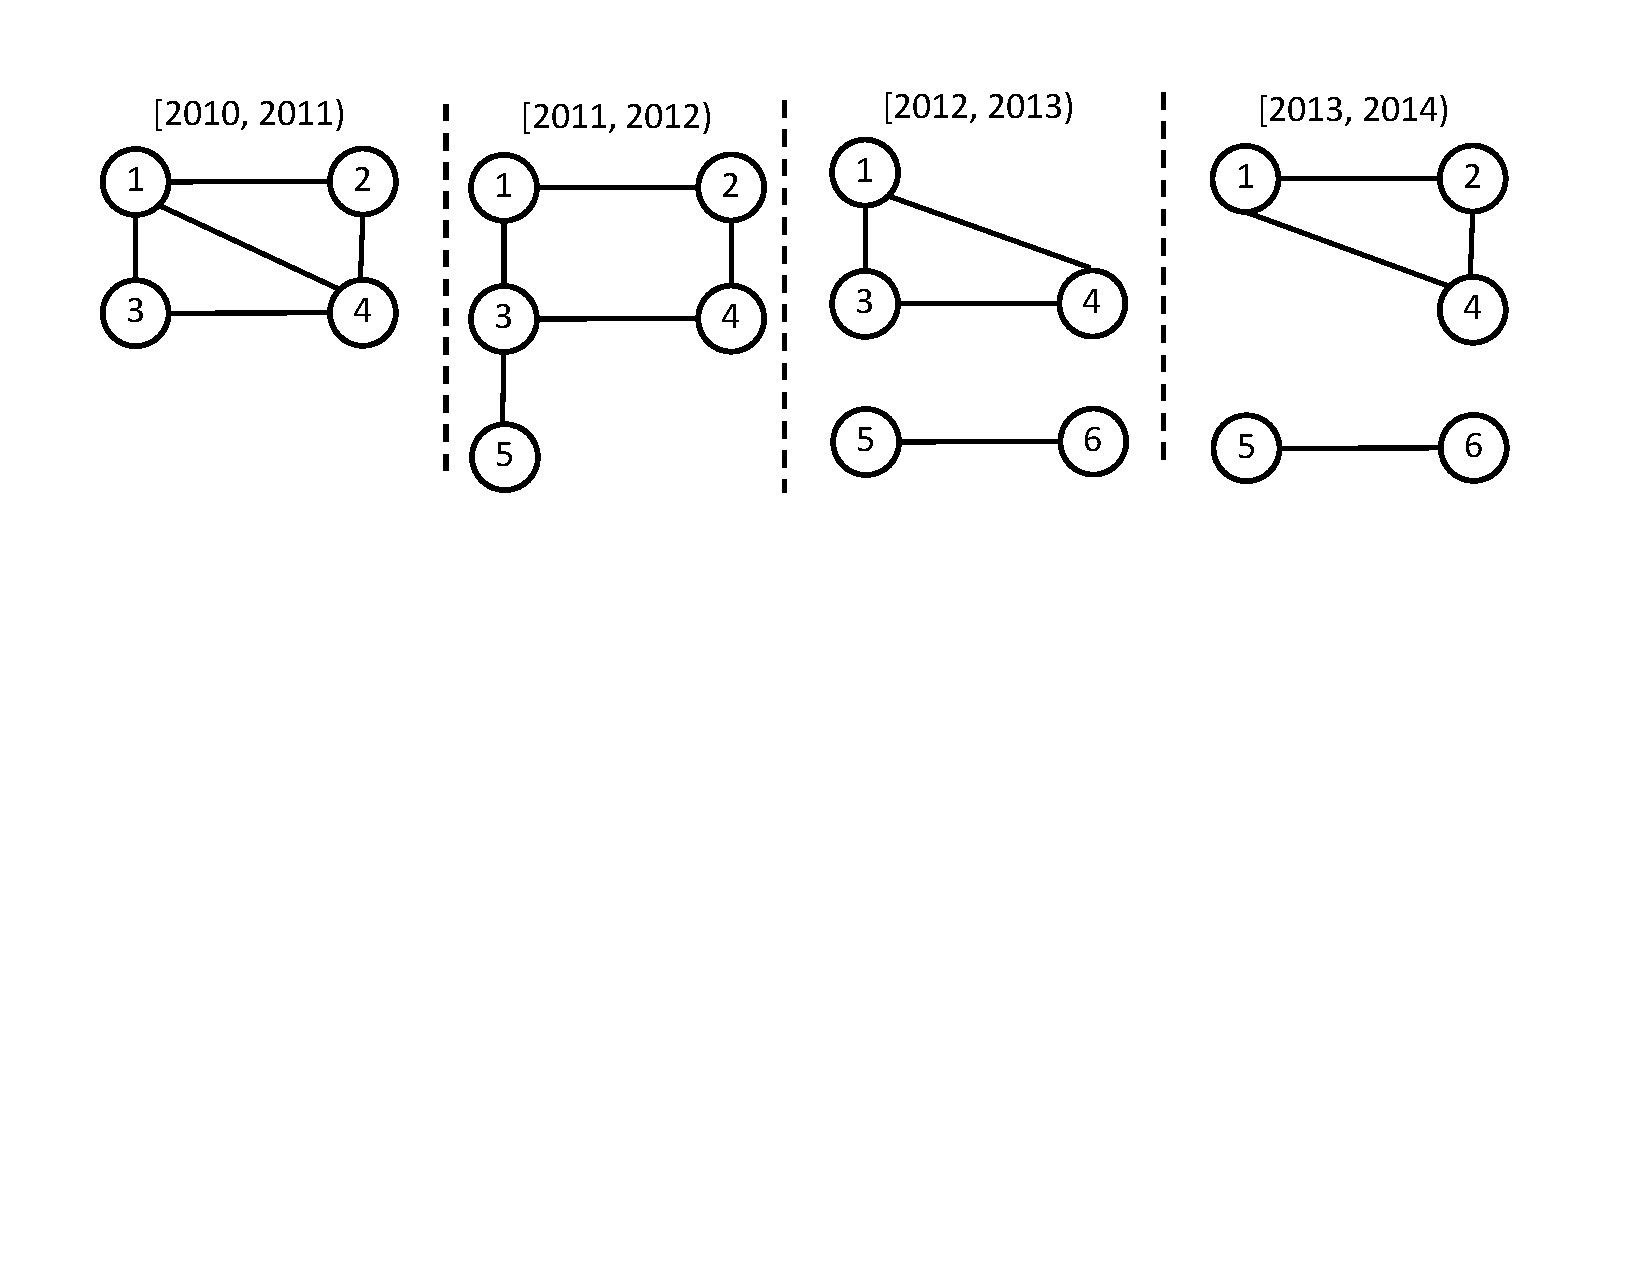
\includegraphics[width=2.9in]{figs/4snaps_T1.pdf}
  \caption{\tg \insql{T1} with 4 snapshots.}{}
\vspace{-0.5cm}
  \label{fig:tg_t1}
\end{minipage}%
\begin{minipage}{3.2in}
%  \centering
  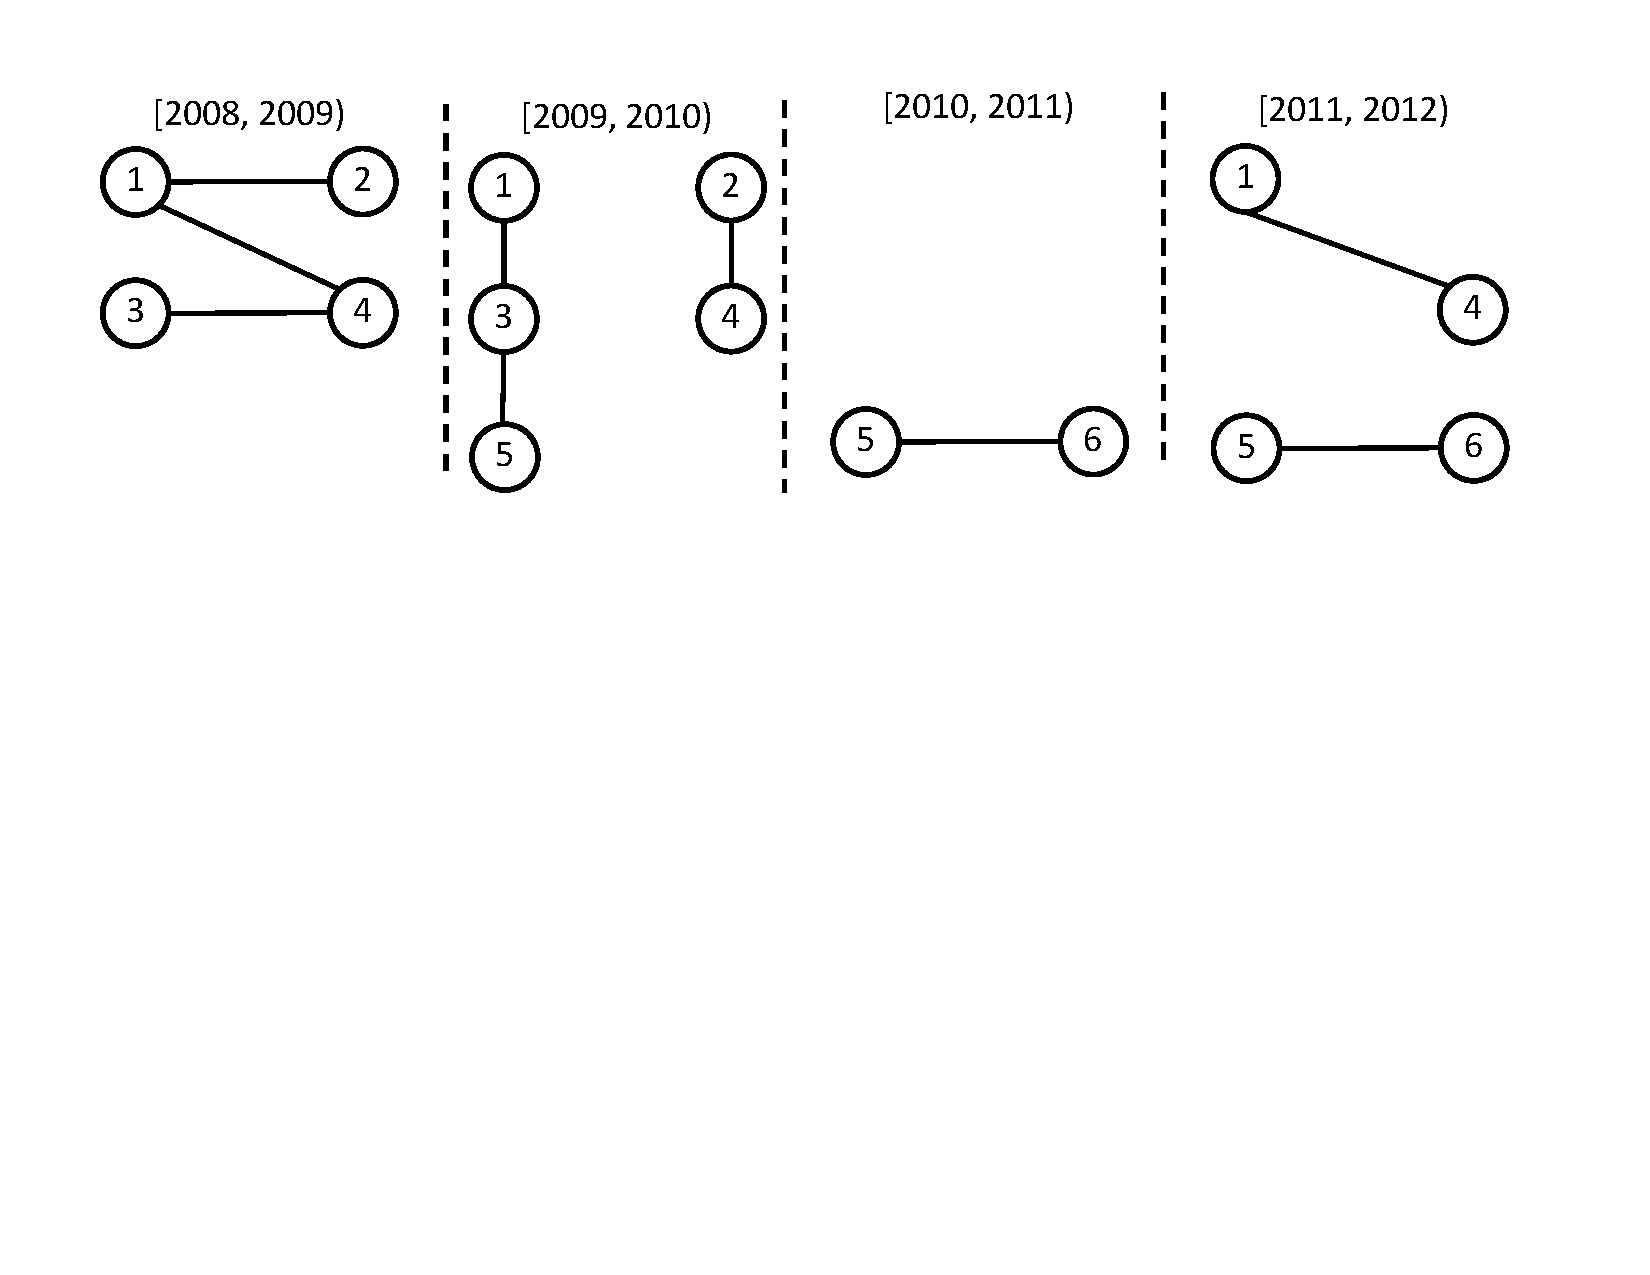
\includegraphics[width=2.9in]{figs/4snaps_T2.pdf}
  \caption{\tg \insql{T2} with 4 snapshots.}{}
\vspace{-0.5cm}
  \label{fig:tg_t2}
\end{minipage}
\end{figure*}
}

\ql is a declarative query language for evolving graphs.  We give a
brief overview of the language here, see~\cite{PortalarXiv2016} for a
detailed description.

\ql operates on a novel kind of a relation, called a \tg, which can be
provided as a base relation or computed as a view.  A \tg associates a
sequence of consecutive non-overlapping open-closed time periods of
the same duration with a sequence of snapshots.  An example of a
4-snapshot \tg is given in Figure~\ref{fig:tg_t1}, with vertex and
edge relations in Figure~\ref{fig:tg_t1_ve}.

\eat{
Our basic abstraction is that of a graph that evolves over time.  A
snapshot represents a single state of an evolving graph, and is not
time-aware.  Temporal evolution of a graph is represented by a
sequence of snapshots, called a {\em temporal graph}, or \tg for
short, with an associated temporal sequence.  A temporal sequence, in
turn, is a sequence of consecutive non-overlapping open-closed time
periods of the same duration.}

\ql supports unary and binary operations on \tgs, and is fully
compositional. \ql uses SQL-like syntax, and has the form
\insql{TSelect} \ldots \insql{From} \ldots \insql{TWhere} \ldots
\insql{TGroup}.  We prefix temporal keywords with \insql{T}, to make
the distinction between \ql and SQL operations explicit. 

\eat{ \ql supports evolving graph-specific operations such as snapshot
  analytics (e.g., pagerank) and temporal aggregation, along with
  generic set-based operations such as a join.}

Consider query \insql{Q1} below.  This query is concise, yet it
specifies a sophisticated analysis task.

\eat{{\footnotesize}}
\begin{small}
\begin{verbatim}
 Q1:  TSelect V [vid, pagerank()] ; 
              E [vid1, vid2, sum(cnt)] 
      From    T1 TOr T2 
      TWhere  Start >= 2010 And End < 2014 
      TGroup  by 2 years
\end{verbatim}
\end{small}
%}

\begin{figure}[t!]
  \centering
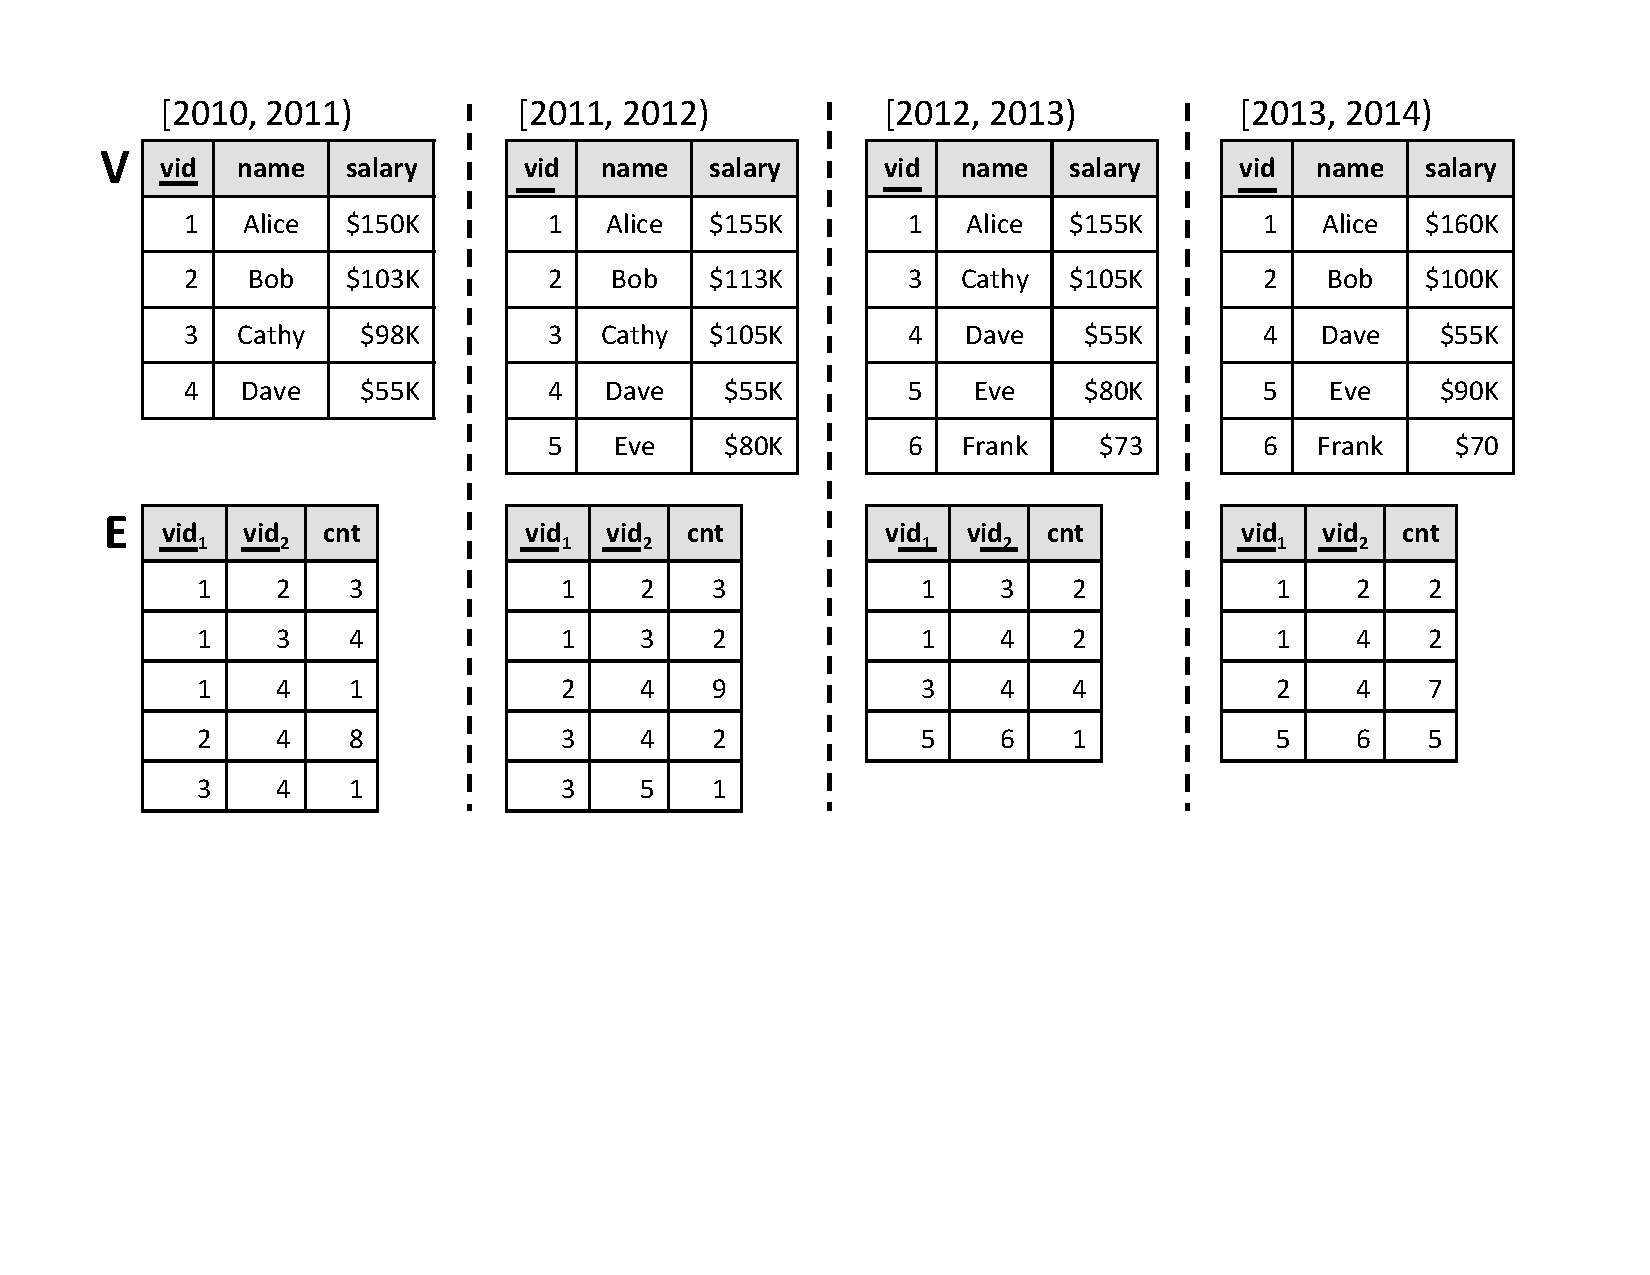
\includegraphics[width=3.5in]{figs/4snaps_T1_ve.pdf}
  \vspace{-0.5cm}
  \caption{Vertex and edge attributes of \tg \insql{T1}.}{}
  \label{fig:tg_t1_ve}
\vspace{-0.3cm}
\end{figure}

\insql{Q1} combines \tgs \insql{T1} and \insql{T2}, restricts the
result to the $[2010, 2014)$ range, groups the result into 2-year
  windows, computes \insql{pagerank()} for each vertex in each time
  window, and sums values of the attribute \insql{cnt} for each edge.

Note the use of \insql{TOr} in \insql{Q1}.  This is one kind of a
temporal join supported in \ql, returning the union of the snapshots
of the two operands.  (\ql also support temporal intersection
\insql{TAnd}, illustrated in \insql{Q2}).  Temporal join is a binary
operation that requires its operands to be {\em union-compatible}.
There are two parts to union-compatibility, structural and temporal.
Structural union-compatibility states that vertex and edge relations
of the two \tgs must be union-compatible.  Temporal
union-compatibility states that temporal sequences of \insql{T1} and
\insql{T2} must have the same resolution, and they must align.

As part of query \insql{Q1}, \ql performs {\em structural
  aggregation}.  This operation is part of temporal aggregation
(\insql{TGroup}) and temporal join (\insql{TOr}).  The default is to
take the union of vertices and edges; it can be over-ridden to compute
an intersection of the edges, or of the vertices, or both.

\ql supports two families of analytics.  The first are snapshot
analytics, which are executed on each graph in a series of
temporally-adjacent snapshots.  The second are trend analytics,
computed across groups of temporally-adjacent snapshots.  Both are
illustrated in \insql{Q2} below.

\eat{{\footnotesize}}
\begin{small}
\begin{verbatim}
Q2:  TSelect V [vid, trend(pr)];
             E [vid1, vid2]  
     From    ( TSelect V [vid, pagerank() as pr];   
                       E [vid1, vid2]
               From    T1 TAnd T2 )
     TGroup  by Size
\end{verbatim}
\end{small}
%}

\insql{Q2} executes a temporal join of \insql{T1} and \insql{T2} and
\eat{, then}invokes \insql{pagerank()}, a {\em snapshot analytic}, on
consecutive snapshots of the result.  Our current focus is on
Pregel-style \eat{snapshot} analytics.  We may accommodate additional
classes \eat{of analytics }in the future.

Consider the use of the {\em trend analytic} function
\insql{trend(pr)}, which aggregates the sequence of PageRank scores of
each vertex.  In our implementation we use a common definition of
\insql{trend}: compute the slope of the least squares line using
linear regression, making an adjustment when a vertex value is
missing.  While this is the only trend analytic we currently support,
we are working on an API that will allow developers to implement
custom trend analytics, taking attributes of both atomic and complex
type as input, and computing a value of either an atomic or a complex
type.


\eat{
For example, consider the following query:

\begin{small}
\begin{verbatim}
Q1:  TSelect Any V [vid, any(name), max(salary)] ; 
             Any E [vid1, vid2, sum(cnt)] 
     From    T1 
     TGroup  by 2 years
\end{verbatim}
\end{small}

\insql{Q1} temporally aggregates snapshots of \tg \insql{T1} into
snapshots in 2 year increments, followed by a projection
($max(salary)$ and $sum(cnt)$ are parts of aggregation).  A more
complex query using 5 operations:

\begin{small}
\begin{verbatim}
Q2:  TSelect Any V [vid, pagerank() as pr] ; 
             Any E [vid1, vid2] 
     From    T1 TAnd T2 
     TWhere  Start >= 2012 And End < 2014 
     TGroup  by 2 years
\end{verbatim}
\end{small}

\insql{Q2} uses temporal join ($TAnd$), followed by temporal selection
($TWhere$), aggregation ($TGroup$), snapshot analytics, and
projection.  For more detail about the language, please see~\cite{}.

}
